% Options for packages loaded elsewhere
\PassOptionsToPackage{unicode}{hyperref}
\PassOptionsToPackage{hyphens}{url}
%
\documentclass[
]{article}
\usepackage{lmodern}
\usepackage{amssymb,amsmath}
\usepackage{ifxetex,ifluatex}
\ifnum 0\ifxetex 1\fi\ifluatex 1\fi=0 % if pdftex
  \usepackage[T1]{fontenc}
  \usepackage[utf8]{inputenc}
  \usepackage{textcomp} % provide euro and other symbols
\else % if luatex or xetex
  \usepackage{unicode-math}
  \defaultfontfeatures{Scale=MatchLowercase}
  \defaultfontfeatures[\rmfamily]{Ligatures=TeX,Scale=1}
\fi
% Use upquote if available, for straight quotes in verbatim environments
\IfFileExists{upquote.sty}{\usepackage{upquote}}{}
\IfFileExists{microtype.sty}{% use microtype if available
  \usepackage[]{microtype}
  \UseMicrotypeSet[protrusion]{basicmath} % disable protrusion for tt fonts
}{}
\makeatletter
\@ifundefined{KOMAClassName}{% if non-KOMA class
  \IfFileExists{parskip.sty}{%
    \usepackage{parskip}
  }{% else
    \setlength{\parindent}{0pt}
    \setlength{\parskip}{6pt plus 2pt minus 1pt}}
}{% if KOMA class
  \KOMAoptions{parskip=half}}
\makeatother
\usepackage{xcolor}
\IfFileExists{xurl.sty}{\usepackage{xurl}}{} % add URL line breaks if available
\IfFileExists{bookmark.sty}{\usepackage{bookmark}}{\usepackage{hyperref}}
\hypersetup{
  hidelinks,
  pdfcreator={LaTeX via pandoc}}
\urlstyle{same} % disable monospaced font for URLs
\usepackage[margin=1in]{geometry}
\usepackage{color}
\usepackage{fancyvrb}
\newcommand{\VerbBar}{|}
\newcommand{\VERB}{\Verb[commandchars=\\\{\}]}
\DefineVerbatimEnvironment{Highlighting}{Verbatim}{commandchars=\\\{\}}
% Add ',fontsize=\small' for more characters per line
\usepackage{framed}
\definecolor{shadecolor}{RGB}{248,248,248}
\newenvironment{Shaded}{\begin{snugshade}}{\end{snugshade}}
\newcommand{\AlertTok}[1]{\textcolor[rgb]{0.94,0.16,0.16}{#1}}
\newcommand{\AnnotationTok}[1]{\textcolor[rgb]{0.56,0.35,0.01}{\textbf{\textit{#1}}}}
\newcommand{\AttributeTok}[1]{\textcolor[rgb]{0.77,0.63,0.00}{#1}}
\newcommand{\BaseNTok}[1]{\textcolor[rgb]{0.00,0.00,0.81}{#1}}
\newcommand{\BuiltInTok}[1]{#1}
\newcommand{\CharTok}[1]{\textcolor[rgb]{0.31,0.60,0.02}{#1}}
\newcommand{\CommentTok}[1]{\textcolor[rgb]{0.56,0.35,0.01}{\textit{#1}}}
\newcommand{\CommentVarTok}[1]{\textcolor[rgb]{0.56,0.35,0.01}{\textbf{\textit{#1}}}}
\newcommand{\ConstantTok}[1]{\textcolor[rgb]{0.00,0.00,0.00}{#1}}
\newcommand{\ControlFlowTok}[1]{\textcolor[rgb]{0.13,0.29,0.53}{\textbf{#1}}}
\newcommand{\DataTypeTok}[1]{\textcolor[rgb]{0.13,0.29,0.53}{#1}}
\newcommand{\DecValTok}[1]{\textcolor[rgb]{0.00,0.00,0.81}{#1}}
\newcommand{\DocumentationTok}[1]{\textcolor[rgb]{0.56,0.35,0.01}{\textbf{\textit{#1}}}}
\newcommand{\ErrorTok}[1]{\textcolor[rgb]{0.64,0.00,0.00}{\textbf{#1}}}
\newcommand{\ExtensionTok}[1]{#1}
\newcommand{\FloatTok}[1]{\textcolor[rgb]{0.00,0.00,0.81}{#1}}
\newcommand{\FunctionTok}[1]{\textcolor[rgb]{0.00,0.00,0.00}{#1}}
\newcommand{\ImportTok}[1]{#1}
\newcommand{\InformationTok}[1]{\textcolor[rgb]{0.56,0.35,0.01}{\textbf{\textit{#1}}}}
\newcommand{\KeywordTok}[1]{\textcolor[rgb]{0.13,0.29,0.53}{\textbf{#1}}}
\newcommand{\NormalTok}[1]{#1}
\newcommand{\OperatorTok}[1]{\textcolor[rgb]{0.81,0.36,0.00}{\textbf{#1}}}
\newcommand{\OtherTok}[1]{\textcolor[rgb]{0.56,0.35,0.01}{#1}}
\newcommand{\PreprocessorTok}[1]{\textcolor[rgb]{0.56,0.35,0.01}{\textit{#1}}}
\newcommand{\RegionMarkerTok}[1]{#1}
\newcommand{\SpecialCharTok}[1]{\textcolor[rgb]{0.00,0.00,0.00}{#1}}
\newcommand{\SpecialStringTok}[1]{\textcolor[rgb]{0.31,0.60,0.02}{#1}}
\newcommand{\StringTok}[1]{\textcolor[rgb]{0.31,0.60,0.02}{#1}}
\newcommand{\VariableTok}[1]{\textcolor[rgb]{0.00,0.00,0.00}{#1}}
\newcommand{\VerbatimStringTok}[1]{\textcolor[rgb]{0.31,0.60,0.02}{#1}}
\newcommand{\WarningTok}[1]{\textcolor[rgb]{0.56,0.35,0.01}{\textbf{\textit{#1}}}}
\usepackage{longtable,booktabs}
% Correct order of tables after \paragraph or \subparagraph
\usepackage{etoolbox}
\makeatletter
\patchcmd\longtable{\par}{\if@noskipsec\mbox{}\fi\par}{}{}
\makeatother
% Allow footnotes in longtable head/foot
\IfFileExists{footnotehyper.sty}{\usepackage{footnotehyper}}{\usepackage{footnote}}
\makesavenoteenv{longtable}
\usepackage{graphicx}
\makeatletter
\def\maxwidth{\ifdim\Gin@nat@width>\linewidth\linewidth\else\Gin@nat@width\fi}
\def\maxheight{\ifdim\Gin@nat@height>\textheight\textheight\else\Gin@nat@height\fi}
\makeatother
% Scale images if necessary, so that they will not overflow the page
% margins by default, and it is still possible to overwrite the defaults
% using explicit options in \includegraphics[width, height, ...]{}
\setkeys{Gin}{width=\maxwidth,height=\maxheight,keepaspectratio}
% Set default figure placement to htbp
\makeatletter
\def\fps@figure{htbp}
\makeatother
\setlength{\emergencystretch}{3em} % prevent overfull lines
\providecommand{\tightlist}{%
  \setlength{\itemsep}{0pt}\setlength{\parskip}{0pt}}
\setcounter{secnumdepth}{5}
\usepackage{graphicx}
\usepackage{hyperref}

\author{}
\date{\vspace{-2.5em}}

\begin{document}

%Turn off page numbering
\pagenumbering{gobble}
\begin{center}

\Huge{Simulations of an impulsive model for the growth of fruit trees}\\
\vspace{\baselineskip}
\LARGE{Theme 08 - Introduction to Systems Biology}\\
\large{Reproduce research}\\
\vspace{\baselineskip}

\begin{figure}
  \centering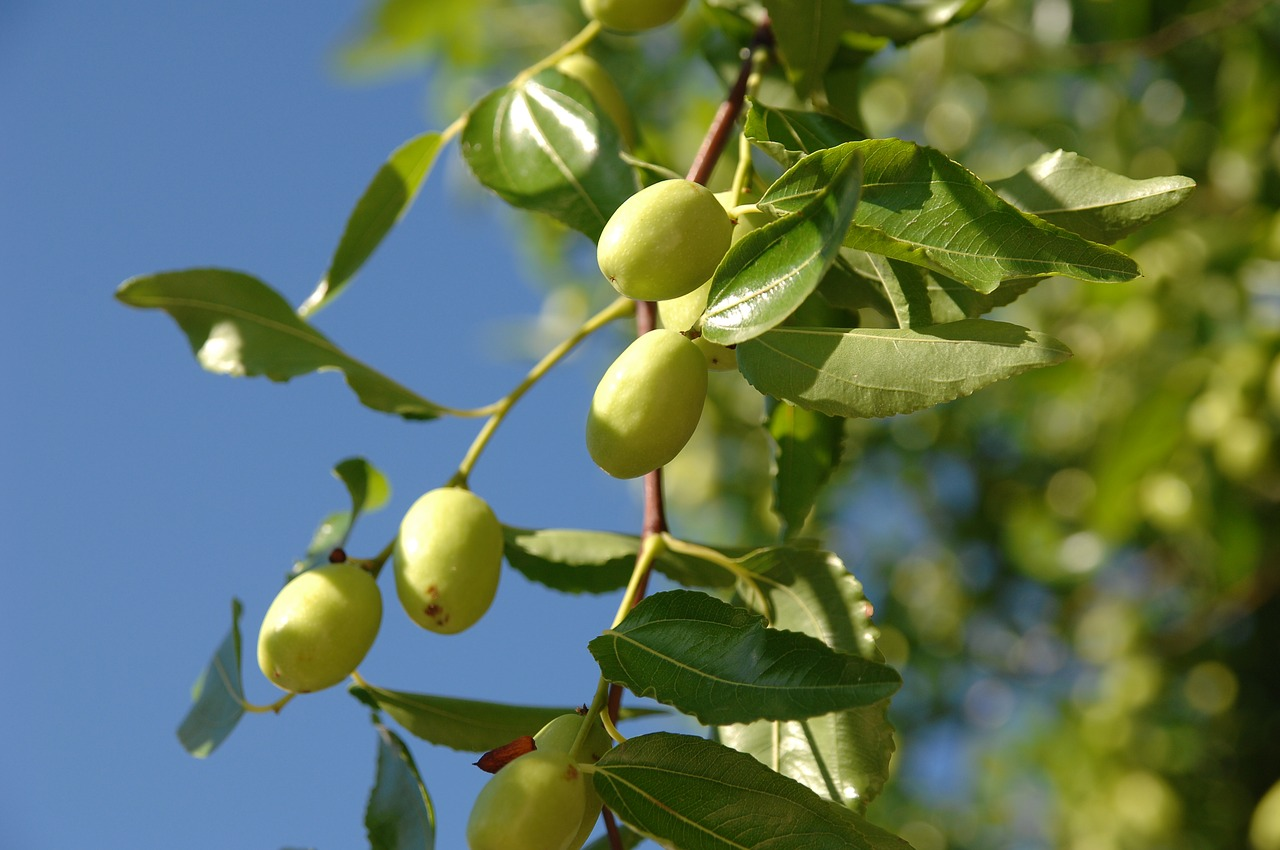
\includegraphics[width=\linewidth]{jujube}
  \label{fig:jujube}
\end{figure}

\end{center}
\vspace{\baselineskip}

%Students info
\normalsize
\vspace*{\fill}
\begin{flushright}
Lisa J.B. Hu (414264)\\
Niek R. Scholten (388602)\\
Bio-Informatics BFV2\\
Institute of Life Science \& Technology\\
Hanze University of Applied Sciences\\
Tsjerk Wassenaar\\
\today
\end{flushright}
\newpage

%Blank page
\null
\thispagestyle{empty}
\addtocounter{page}{-1}
\newpage

\begin{center}

%Titles

\Huge{Simulations of an impulsive model for the growth of fruit trees}\\
\vspace{\baselineskip}
\LARGE{Theme 08 - Introduction to Systems Biology}\\
\vspace{\baselineskip}

\end{center}
\vspace{\baselineskip}

%Students info
\normalsize
\vspace*{\fill}
\begin{flushright}
Lisa J.B. Hu (414264)\\
Niek R. Scholten (388602)\\
Bio-Informatics BFV2\\
Institute of Life Science \& Technology\\
Hanze University of Applied Sciences\\
Tsjerk Wassenaar\\
\today
\end{flushright}
\newpage

\pagenumbering{roman}
\section*{Abstract}

Droughts have affected the agriculture in the mediterranean in an increasingly severe matter.
The decrease in rainfall and the effects of global warming have taken their toll on many orchards, especially fruit producing ones.
Since the water supply of these orchards is always artificial because of the aforementioned factors, dwindling water capacities in reservoirs is a serious issue.
This study aims to provide an insight into the effects of different irrigation patterns on the growth of these fruit trees.
Without a sustainable plan for irrigation, whole populations of fruit trees might perish under a critical water deficit.

\label{sec:abstract}~\addcontentsline{toc}{section}{\nameref{sec:abstract}}
\newpage

\section*{Summary}
test section
\label{sec:summ}~\addcontentsline{toc}{section}{\nameref{sec:summ}}
\newpage

\section*{List of Abbreviations}

\textbf{ODE} Ordinary Differential Equation

\label{sec:abvs}~\addcontentsline{toc}{section}{\nameref{sec:abvs}}

\newpage

{
\setcounter{tocdepth}{2}
\tableofcontents
}
\newpage

\pagenumbering{arabic}

\hypertarget{introduction}{%
\section{Introduction}\label{introduction}}

\hypertarget{purpose}{%
\subsection{Purpose}\label{purpose}}

The effects of climate change are an existential threat to planet earth.
This paper's purpose is to reproduce and expand on the research done by
E Duque-Marin to get a further understanding of the dynamics and
different scenarios of fruit tree growth, and by extension shed light on
a part of this humongous problem that is already cropping up around the
world.

\hypertarget{theory}{%
\subsection{Theory}\label{theory}}

The growth of the fruit tree is highly impacted by the different
variables in- and outside the tree. To construct an impulsive model, an
order of assumptions must be made:

\begin{enumerate}
\def\labelenumi{\arabic{enumi}.}
\tightlist
\item
  The growth dynamics is governed by an interaction between the
  variables energy, water, vegetative growth.
\item
  The fruit tree responds instantly to the irrigation application.
\item
  The model concerned an adult fruit tree (older than 5 years) with a
  suitable soil surface for the growth of the fruit tree.
\item
  Ideal agronomic management conditions.
\item
  Optimal environmental conditions: The energy of the system is
  constant.
\end{enumerate}

The parameters concerning the model are summarized in Table
\ref{tab:tab1}.

\begin{longtable}[]{@{}ll@{}}
\caption{Parameters used for the model \label{tab:tab1}}\tabularnewline
\toprule
\textbf{Parameter} & \textbf{Meaning}\tabularnewline
\midrule
\endfirsthead
\toprule
\textbf{Parameter} & \textbf{Meaning}\tabularnewline
\midrule
\endhead
\(q\) & Accumulated energy constant\tabularnewline
\(r\) & Fruit trees intrinsic growth rate\tabularnewline
\(N\) & Fruit carrying capacity\tabularnewline
\(I\) & Irrigation water amount\tabularnewline
\(\beta\) & Evapotranspiration rate\tabularnewline
\(\gamma\) & Photosynthetic contribution rate\tabularnewline
\(\omega\) & Mortality rate of fruit trees\tabularnewline
\bottomrule
\end{longtable}

With that, the state variables can be denoted as following:

\begin{enumerate}
\def\labelenumi{\arabic{enumi}.}
\tightlist
\item
  \emph{E = E(t)} the solar radiation at time \emph{t};
\item
  \emph{W = W(t)} the water amount in the soil at time \emph{t};
\item
  \emph{C = C(t)} the fruit biomass concentration at time \emph{t}.
\end{enumerate}

Under assumption 5, the state variables are reduced to only \emph{W} and
\emph{C}. The variation of the amount of water in the system is denoted
by \emph{W'(t)} and the variation in biomass is denoted by \emph{C'(t)}.
Considering there is no rainfall (p = 0), the water variation output is
due to evapotranspiration at rate \(\beta\). Besides that, water is
crucial for promoting the growth of the fruit tree at rate \(r\).

C'(t) corresponds to the water input at a rate \(r\); in addition, it is
also positively affected due to the water-energy-biomass growth
interaction at a rate \(\gamma\). There is an exit at an \(\omega\) rate
for the loss of natural death of the crop. This behavior applies to a
continuous timescale (long duration), that governs the growth dynamics
of the fruit tree. However, this model also presents a short timescale
(pulse) in discrete time that represents the events in which water
enters the system through irrigation supply.

The dynamics between the variables energy, amount of water, and
concentration of biomass of the fruit tree are shown in Figure
\ref{fig:fig1}, adapted from \ref{ref:ref1}; where: \emph{E} = Energy;
\emph{W} = Water amount; \emph{C} = Fruit biomass concentration; \(r\) =
Fruit trees intrinsic growth rate; \emph{N} = Fruit carrying capacity;
\(\beta\) = Evapotranspiration rate; \(\gamma\) = Photosynthetic
contribution rate; \(\omega\) = Mortality rate of fruit trees; \(p\) =
Rainfall rate; \emph{I} = Irrigation amount.\newline

\begin{figure}

{\centering 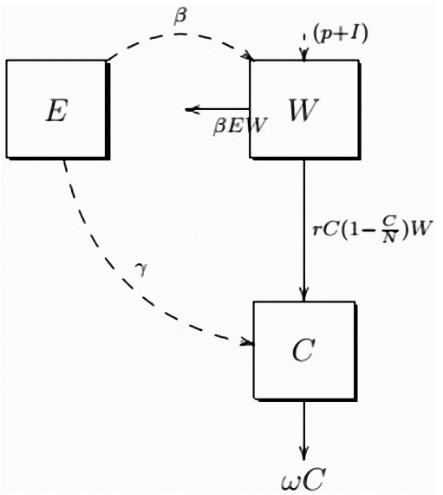
\includegraphics[width=0.5\linewidth]{dynamics} 

}

\caption{\label{fig:fig1}Diagram of dynamics}\label{fig:unnamed-chunk-1}
\end{figure}

A model can be proposed that represents the growth dynamics of fruit
trees, where the supply of irrigation is evidenced in the form of a
pulse, and thus be described by impulsive differential equations
\ref{eq:eq1}.

Equations: \[
  \begin{array}{cc}
  W'(t) = -\beta qW(t) - rC(t)(1 - \frac{C(t)}{N} W(t) & \\
  C'(t) = rC(t)(1 - \frac{C(t)}{N})W(t) + \frac{\gamma qC(t)W(t)}{(C+1)(W+1)}-\omega C(1) & t \ne nT\\
  \Delta W(nT) = I & \\
  \Delta C(nT) = 0 & t = nT\\
  \end{array}
\] \hfill (\label{eq:eq1}1.2)

\newpage

\hypertarget{materials-and-methods}{%
\section{Materials and Methods}\label{materials-and-methods}}

Since no datasets were used in the production of the results, the
simulation data had to be generated. This data was plotted using R
graphics.

\hypertarget{materials}{%
\subsection{Materials}\label{materials}}

The simulation data was obtained using the ODE (ordinary differential
equation) function of the deSolve package. This function takes
differential equations and parameters and calculates the output of these
functions. Aforementioned equations can ben found in the theory section.
Other packages like ggplot2, ggpubr, formatR and scales were used in
data visualisation. (\ref{tab:tab2})

\begin{longtable}[]{@{}lll@{}}
\caption{Software and packages \label{tab:tab2}}\tabularnewline
\toprule
\textbf{Software} & \textbf{Package} & \textbf{Version}\tabularnewline
\midrule
\endfirsthead
\toprule
\textbf{Software} & \textbf{Package} & \textbf{Version}\tabularnewline
\midrule
\endhead
R & & 4.0.4\tabularnewline
& deSolve & 1.32\tabularnewline
& formatR & 1.11.1\tabularnewline
& ggplot2 & 3.3.5\tabularnewline
& ggpubr & 0.4.0\tabularnewline
& scales & 1.1.1\tabularnewline
\bottomrule
\end{longtable}

The simulation data consists of an index, the \(time\), water level in
the soil (\(W\)) and biomass (\(C\)). (\ref{tab:tab3})

\begin{longtable}[]{@{}llll@{}}
\caption{The simulation data \label{tab:tab3}}\tabularnewline
\toprule
& \textbf{\(time\)} & \textbf{\(W\)} & \textbf{\(C\)}\tabularnewline
\midrule
\endfirsthead
\toprule
& \textbf{\(time\)} & \textbf{\(W\)} & \textbf{\(C\)}\tabularnewline
\midrule
\endhead
1 & 0.00000 & 0.600000 & 1.00000\tabularnewline
2 & 1.00000 & 0.556209 & 1.02602\tabularnewline
3 & 2.00000 & 0.514991 & 1.05076\tabularnewline
4 & 3.00000 & 0.476281 & 1.07421\tabularnewline
5 & 4.00000 & 0.440001 & 1.09637\tabularnewline
\bottomrule
\end{longtable}

\hypertarget{methods}{%
\subsection{Methods}\label{methods}}

The differential equations were translated into a mathematical model
that deSolve could understand. The last two equations also needed to be
incorporated; this was done through if/else statements checking the
timestep. After several tests were run to ensure parity with the
described model in the paper. See Appendix \ref{appendix-b}

After this, the model was updated to use one-hour steps instead of
one-day steps. This lead to the model being adapted to incorporate
different growth rates for day and night, for even more precise data.
See Appendix \ref{appendix-c}.

Another few models were made to compare different irrigation intervals,
as well as a model for watering the soil as soon as almost all water was
drained from it. See Appendix \ref{appendix-d} and \ref{appendix-e}.

\newpage

\hypertarget{results}{%
\section{Results}\label{results}}

\hypertarget{replication}{%
\subsection{Replication}\label{replication}}

The growth of the fruit trees can be shown in multiple simulations,
tweaking a few variables to see the differences between these. In Figure
\ref{fig:fig2}a, the courses of the two state variables are shown: The
water amount in the soil (blue) and the growth of the fruit tree's
biomass (red). Figure \ref{fig:fig2}b shows what happens with the growth
of the fruit tree if the parameter \emph{q} changes, for \(q = 0.1\) in
red, \(q = 0.5\) in black (the default value), and \(q = 1\) in blue.

\begin{figure}
\centering
\includegraphics{/home/nieks/PycharmProjects/Bio-Informatica-Hanze/Thema 08 - Introduction to Systems Biology/Praktijkopdracht/Final/final_report_files/figure-latex/res1-1.pdf}
\caption{\label{fig:fig2}The different simulations}
\end{figure}

\newpage

\hypertarget{expansion}{%
\subsection{Expansion}\label{expansion}}

The following simulations show the difference between the expanded model
accounting for day and night cycles in red, and the original model from
\ref{ref:ref1} in black. Figure \ref{fig:fig3} shows a decrease in
overall biomass production, while steady growth is still retained. This
change has to do with the fact that a little under half of a 24-hour
period is calculated as ``no growth'' night-time.

\begin{figure}
\centering
\includegraphics{/home/nieks/PycharmProjects/Bio-Informatica-Hanze/Thema 08 - Introduction to Systems Biology/Praktijkopdracht/Final/final_report_files/figure-latex/res2-1.pdf}
\caption{\label{fig:fig3}The expanded simulation}
\end{figure}

\newpage

\hypertarget{comparison}{%
\subsection{Comparison}\label{comparison}}

Comparing different sets of irrigation data is vital to understanding
the most efficient way of watering the fruit trees. Figure
\ref{fig:fig4} shows the difference between the reference research from
the paper and newly run simulations.

\begin{figure}
\centering
\includegraphics{/home/nieks/PycharmProjects/Bio-Informatica-Hanze/Thema 08 - Introduction to Systems Biology/Praktijkopdracht/Final/final_report_files/figure-latex/res3-1.pdf}
\caption{\label{fig:fig4}The simulation comparisons}
\end{figure}

\newpage

\hypertarget{desiccation}{%
\subsection{Desiccation}\label{desiccation}}

\begin{figure}
\centering
\includegraphics{/home/nieks/PycharmProjects/Bio-Informatica-Hanze/Thema 08 - Introduction to Systems Biology/Praktijkopdracht/Final/final_report_files/figure-latex/res4-1.pdf}
\caption{\label{fig:fig5}The edge case simulation}
\end{figure}

\newpage

\hypertarget{conclusion}{%
\section{Conclusion}\label{conclusion}}

In this work, simulations of an impulsive system of nonlinear
differential equations were reproduced to describe the growth of fruit
trees when exposed the application of water by irrigation. These models
were then expanded upon to incorporate day/night cycles for the trees to
respond to. The results of this work not only exhibit the positive
effects of a well scheduled irrigation system, but also the negative
effects of a system that is not well scheduled. Results like these are
very important factors in addressing problems that have to do with
climate change induced drought. All this culminates into the conclusion
that artificial irrigation is an essential part of growing fruit trees
in areas with frequent drought and decreasing rainfall as an effect of
climate change.

\newpage

\hypertarget{discussion}{%
\section{Discussion}\label{discussion}}

\newpage

\hypertarget{references}{%
\section{References}\label{references}}

\newpage

\hypertarget{appendix}{%
\section{Appendix}\label{appendix}}

\hypertarget{appendix-a}{%
\subsection{Appendix A}\label{appendix-a}}

\begin{Shaded}
\begin{Highlighting}[numbers=left,,]
\CommentTok{\#\# {-}{-}{-}{-}{-}{-}{-}{-}{-}{-}{-}{-}{-}{-}{-}{-}{-}{-}{-}{-}{-}{-}{-}{-}{-}{-}{-}}
\CommentTok{\#\#}
\CommentTok{\#\# Name: functions.R}
\CommentTok{\#\#}
\CommentTok{\#\# Author: Lisa Hu}
\CommentTok{\#\#}
\CommentTok{\#\# Purpose: Script contains functions used in the result scripts}
\CommentTok{\#\#}
\CommentTok{\#\# Email: l.j.b.hu@st.hanze.nl}
\CommentTok{\#\#}
\CommentTok{\#\# {-}{-}{-}{-}{-}{-}{-}{-}{-}{-}{-}{-}{-}{-}{-}{-}{-}{-}{-}{-}{-}{-}{-}{-}{-}{-}{-}}

\CommentTok{\#\# {-}{-}{-}{-} basic{-}model}
\NormalTok{model \textless{}{-}}\StringTok{ }\ControlFlowTok{function}\NormalTok{(t, y, parms)\{}
  \CommentTok{\# Add water every given days, until day 80}
  \ControlFlowTok{if}\NormalTok{(t }\OperatorTok{\%\%}\StringTok{ }\KeywordTok{as.numeric}\NormalTok{(parms[}\StringTok{"time"}\NormalTok{]) }\OperatorTok{==}\StringTok{ }\DecValTok{0} \OperatorTok{\&\&}\StringTok{ }\NormalTok{t }\OperatorTok{\textless{}}\StringTok{ }\DecValTok{80} \OperatorTok{\&\&}\StringTok{ }\NormalTok{t }\OperatorTok{\textgreater{}}\StringTok{ }\DecValTok{0}\NormalTok{)\{}
    \KeywordTok{with}\NormalTok{(}\KeywordTok{as.list}\NormalTok{(}\KeywordTok{c}\NormalTok{(parms, y)), \{}
\NormalTok{      dW \textless{}{-}}\StringTok{ }\NormalTok{I }\CommentTok{\# I is the water irrigation}
\NormalTok{      dC \textless{}{-}}\StringTok{ }\DecValTok{0} \CommentTok{\# There is no growth on those days}
      \KeywordTok{return}\NormalTok{( }\KeywordTok{list}\NormalTok{( }\KeywordTok{c}\NormalTok{(dW, dC) ) )}
\NormalTok{    \})}
\NormalTok{  \}}
  \CommentTok{\# Else the model runs with the equations}
  \ControlFlowTok{else}\NormalTok{\{}
    \KeywordTok{with}\NormalTok{(}\KeywordTok{as.list}\NormalTok{(}\KeywordTok{c}\NormalTok{(parms, y)),\{}
\NormalTok{      dW \textless{}{-}}\StringTok{ }\NormalTok{(}\OperatorTok{{-}}\NormalTok{B }\OperatorTok{*}\StringTok{ }\NormalTok{q }\OperatorTok{*}\StringTok{ }\NormalTok{W) }\OperatorTok{{-}}\StringTok{ }\NormalTok{(r }\OperatorTok{*}\StringTok{ }\NormalTok{C }\OperatorTok{*}\StringTok{ }\NormalTok{(}\DecValTok{1} \OperatorTok{{-}}\StringTok{ }\NormalTok{( C}\OperatorTok{/}\NormalTok{N ) ) }\OperatorTok{*}\StringTok{ }\NormalTok{W)}
\NormalTok{      dC \textless{}{-}}\StringTok{ }\NormalTok{(r }\OperatorTok{*}\StringTok{ }\NormalTok{C }\OperatorTok{*}\StringTok{ }\NormalTok{(}\DecValTok{1} \OperatorTok{{-}}\StringTok{ }\NormalTok{( C}\OperatorTok{/}\NormalTok{N ) ) }\OperatorTok{*}\StringTok{ }\NormalTok{W) }\OperatorTok{+}\StringTok{ }\NormalTok{( (g}\OperatorTok{*}\NormalTok{q}\OperatorTok{*}\NormalTok{C}\OperatorTok{*}\NormalTok{W)}\OperatorTok{/}\NormalTok{(C}\OperatorTok{+}\DecValTok{1}\NormalTok{)}\OperatorTok{*}\NormalTok{(W}\OperatorTok{+}\DecValTok{1}\NormalTok{) ) }\OperatorTok{{-}}\StringTok{ }\NormalTok{o }\OperatorTok{*}\StringTok{ }\NormalTok{C}
      \KeywordTok{return}\NormalTok{( }\KeywordTok{list}\NormalTok{( }\KeywordTok{c}\NormalTok{(dW, dC) ) )}
\NormalTok{    \})}
\NormalTok{  \}}
\NormalTok{\}}

\CommentTok{\#\# {-}{-}{-}{-} Day{-}night model}
\NormalTok{day.night\_model \textless{}{-}}\StringTok{ }\ControlFlowTok{function}\NormalTok{(t, y, parms)\{}
  \CommentTok{\# Add water every given days, until day 80}
  \ControlFlowTok{if}\NormalTok{(t }\OperatorTok{\%\%}\StringTok{ }\KeywordTok{as.numeric}\NormalTok{(parms[}\StringTok{"time"}\NormalTok{]) }\OperatorTok{==}\StringTok{ }\DecValTok{0} \OperatorTok{\&\&}\StringTok{ }\NormalTok{t }\OperatorTok{\textless{}}\StringTok{ }\DecValTok{80} \OperatorTok{\&\&}\StringTok{ }\NormalTok{t }\OperatorTok{\textgreater{}}\StringTok{ }\DecValTok{0}\NormalTok{)\{}
    \KeywordTok{with}\NormalTok{( }\KeywordTok{as.list}\NormalTok{( }\KeywordTok{c}\NormalTok{(parms, y)), \{}
\NormalTok{      dW \textless{}{-}}\StringTok{ }\NormalTok{I }\OperatorTok{*}\StringTok{ }\DecValTok{24} \CommentTok{\# I is the water irrigation}
      \CommentTok{\# }\AlertTok{NOTE}\CommentTok{ : x24 because the water amount should not change}
\NormalTok{      dC \textless{}{-}}\StringTok{ }\DecValTok{0} \CommentTok{\# There is no growth on those days}
      \KeywordTok{return}\NormalTok{( }\KeywordTok{list}\NormalTok{( }\KeywordTok{c}\NormalTok{(dW, dC) ) )}
\NormalTok{    \})}
\NormalTok{  \}}
  \CommentTok{\# Else the model runs with the equations}
  \ControlFlowTok{else}\NormalTok{\{}
    \ControlFlowTok{if}\NormalTok{(t }\OperatorTok{\%\%}\StringTok{ }\DecValTok{1} \OperatorTok{\textless{}=}\StringTok{ }\FloatTok{0.25} \OperatorTok{|}\StringTok{ }\NormalTok{t }\OperatorTok{\%\%}\StringTok{ }\DecValTok{1} \OperatorTok{\textgreater{}=}\StringTok{ }\FloatTok{0.83}\NormalTok{)\{}
      \CommentTok{\# During the night (no sun)}
      \KeywordTok{with}\NormalTok{( }\KeywordTok{as.list}\NormalTok{ (}\KeywordTok{c}\NormalTok{(parms, y)), \{}
\NormalTok{        dW \textless{}{-}}\StringTok{ }\NormalTok{((}\OperatorTok{{-}}\NormalTok{B }\OperatorTok{*}\StringTok{ }\NormalTok{q }\OperatorTok{*}\StringTok{ }\NormalTok{W) }\OperatorTok{{-}}\StringTok{ }\NormalTok{(r }\OperatorTok{*}\StringTok{ }\NormalTok{C }\OperatorTok{*}\StringTok{ }\NormalTok{(}\DecValTok{1} \OperatorTok{{-}}\StringTok{ }\NormalTok{( C}\OperatorTok{/}\NormalTok{N ) ) }\OperatorTok{*}\StringTok{ }\NormalTok{W)) }\CommentTok{\# Normal water drop}
\NormalTok{        dC \textless{}{-}}\StringTok{ }\DecValTok{0} \CommentTok{\# No growth}
        \KeywordTok{return}\NormalTok{( }\KeywordTok{list}\NormalTok{( }\KeywordTok{c}\NormalTok{(dW, dC) ) )}
\NormalTok{        \})}
\NormalTok{    \}}
    \ControlFlowTok{else}\NormalTok{\{}
      \CommentTok{\# During the day (sun)}
      \KeywordTok{with}\NormalTok{( }\KeywordTok{as.list}\NormalTok{( }\KeywordTok{c}\NormalTok{(parms, y)),\{}
\NormalTok{      dW \textless{}{-}}\StringTok{ }\NormalTok{((}\OperatorTok{{-}}\NormalTok{B }\OperatorTok{*}\StringTok{ }\NormalTok{q }\OperatorTok{*}\StringTok{ }\NormalTok{W) }\OperatorTok{{-}}\StringTok{ }\NormalTok{(r }\OperatorTok{*}\StringTok{ }\NormalTok{C }\OperatorTok{*}\StringTok{ }\NormalTok{(}\DecValTok{1} \OperatorTok{{-}}\StringTok{ }\NormalTok{( C}\OperatorTok{/}\NormalTok{N ) ) }\OperatorTok{*}\StringTok{ }\NormalTok{W))}
\NormalTok{      dC \textless{}{-}}\StringTok{ }\NormalTok{((r }\OperatorTok{*}\StringTok{ }\NormalTok{C }\OperatorTok{*}\StringTok{ }\NormalTok{(}\DecValTok{1} \OperatorTok{{-}}\StringTok{ }\NormalTok{( C}\OperatorTok{/}\NormalTok{N ) ) }\OperatorTok{*}\StringTok{ }\NormalTok{W) }\OperatorTok{+}\StringTok{ }\NormalTok{( (g}\OperatorTok{*}\NormalTok{q}\OperatorTok{*}\NormalTok{C}\OperatorTok{*}\NormalTok{W)}\OperatorTok{/}\NormalTok{(C}\OperatorTok{+}\DecValTok{1}\NormalTok{)}\OperatorTok{*}\NormalTok{(W}\OperatorTok{+}\DecValTok{1}\NormalTok{) ) }\OperatorTok{{-}}\StringTok{ }\NormalTok{o }\OperatorTok{*}\StringTok{ }\NormalTok{C)}
      \KeywordTok{return}\NormalTok{( }\KeywordTok{list}\NormalTok{( }\KeywordTok{c}\NormalTok{(dW, dC) ) )}
\NormalTok{      \})}
\NormalTok{    \}}
\NormalTok{  \}}
\NormalTok{\}}

\CommentTok{\#\# {-}{-}{-}{-} water{-}model}
\NormalTok{water\_model \textless{}{-}}\StringTok{ }\ControlFlowTok{function}\NormalTok{(t, y, parms)\{}
  \CommentTok{\# Add water every given days, until day 80}
  \KeywordTok{with}\NormalTok{(}\KeywordTok{as.list}\NormalTok{(}\KeywordTok{c}\NormalTok{(parms, y)),\{}
\NormalTok{    dW \textless{}{-}}\StringTok{ }\NormalTok{(}\OperatorTok{{-}}\NormalTok{B }\OperatorTok{*}\StringTok{ }\NormalTok{q }\OperatorTok{*}\StringTok{ }\NormalTok{W) }\OperatorTok{{-}}\StringTok{ }\NormalTok{(r }\OperatorTok{*}\StringTok{ }\NormalTok{C }\OperatorTok{*}\StringTok{ }\NormalTok{(}\DecValTok{1} \OperatorTok{{-}}\StringTok{ }\NormalTok{( C}\OperatorTok{/}\NormalTok{N ) ) }\OperatorTok{*}\StringTok{ }\NormalTok{W)}
\NormalTok{    dC \textless{}{-}}\StringTok{ }\NormalTok{(r }\OperatorTok{*}\StringTok{ }\NormalTok{C }\OperatorTok{*}\StringTok{ }\NormalTok{(}\DecValTok{1} \OperatorTok{{-}}\StringTok{ }\NormalTok{( C}\OperatorTok{/}\NormalTok{N ) ) }\OperatorTok{*}\StringTok{ }\NormalTok{W) }\OperatorTok{+}\StringTok{ }\NormalTok{( (g}\OperatorTok{*}\NormalTok{q}\OperatorTok{*}\NormalTok{C}\OperatorTok{*}\NormalTok{W)}\OperatorTok{/}\NormalTok{(C}\OperatorTok{+}\DecValTok{1}\NormalTok{)}\OperatorTok{*}\NormalTok{(W}\OperatorTok{+}\DecValTok{1}\NormalTok{) ) }\OperatorTok{{-}}\StringTok{ }\NormalTok{o }\OperatorTok{*}\StringTok{ }\NormalTok{C}
\NormalTok{    dI \textless{}{-}}\StringTok{ }\DecValTok{0}
    \KeywordTok{return}\NormalTok{( }\KeywordTok{list}\NormalTok{( }\KeywordTok{c}\NormalTok{(dW, dC, dI) ) )}
\NormalTok{  \})}
\NormalTok{\}}

\CommentTok{\#\# Function to create plots}
\NormalTok{create.plots \textless{}{-}}\StringTok{ }\ControlFlowTok{function}\NormalTok{(plot.values, ref.data, change.data)\{}
  \CommentTok{\#\textquotesingle{} plot.values = The column name of the datas}
  \CommentTok{\#\textquotesingle{} ref.data = The reference data}
  \CommentTok{\#\textquotesingle{} change.data = The data that contains changed values}
\NormalTok{  data.names \textless{}{-}}\StringTok{ }\KeywordTok{names}\NormalTok{(change.data)}
  \CommentTok{\# Create colours for the different lines (except the reference data)}
\NormalTok{  colours \textless{}{-}}\StringTok{ }\KeywordTok{hue\_pal}\NormalTok{()(}\KeywordTok{length}\NormalTok{(change.data))}
  \CommentTok{\# y.val inserts the plot.value for the corresponding row of data.values}
\NormalTok{  y.val \textless{}{-}}\StringTok{ }\NormalTok{data.values[plot.values,]}
  \CommentTok{\# The plot}
\NormalTok{  plt \textless{}{-}}\StringTok{ }\KeywordTok{ggplot}\NormalTok{(}\DataTypeTok{data =}\NormalTok{ ref.data, }\DataTypeTok{mapping =} \KeywordTok{aes}\NormalTok{(}\DataTypeTok{x =}\NormalTok{ time, }\DataTypeTok{y =} \OperatorTok{!!}\KeywordTok{sym}\NormalTok{(y.val}\OperatorTok{$}\NormalTok{name) ) ) }\OperatorTok{+}
\StringTok{    }\CommentTok{\# Lines (Reference data stays black)}
\StringTok{    }\KeywordTok{geom\_line}\NormalTok{(}\KeywordTok{aes}\NormalTok{(}\DataTypeTok{color =} \StringTok{"Reference"}\NormalTok{)) }\OperatorTok{+}
\StringTok{    }\KeywordTok{unlist}\NormalTok{( }\KeywordTok{mapply}\NormalTok{(}\ControlFlowTok{function}\NormalTok{(single.data, data.name)}
                        \KeywordTok{geom\_line}\NormalTok{(}\DataTypeTok{data =}\NormalTok{ single.data, }\KeywordTok{aes}\NormalTok{(}\DataTypeTok{color =}\NormalTok{ data.name) ),}
\NormalTok{                   change.data, data.names ) ) }\OperatorTok{+}
\StringTok{    }\CommentTok{\# Labels}
\StringTok{    }\KeywordTok{labs}\NormalTok{(}\DataTypeTok{x =} \StringTok{"Time"}\NormalTok{, }\DataTypeTok{y =}\NormalTok{ y.val}\OperatorTok{$}\NormalTok{ylabel) }\OperatorTok{+}
\StringTok{    }\KeywordTok{theme}\NormalTok{(}\DataTypeTok{legend.position =} \StringTok{"bottom"}\NormalTok{) }\OperatorTok{+}
\StringTok{    }\CommentTok{\# Line colours}
\StringTok{    }\KeywordTok{scale\_colour\_manual}\NormalTok{(}\DataTypeTok{values =} \KeywordTok{c}\NormalTok{(}\StringTok{"black"}\NormalTok{, colours),}
                        \DataTypeTok{limits =} \KeywordTok{c}\NormalTok{(}\StringTok{"Reference"}\NormalTok{, }\KeywordTok{names}\NormalTok{(change.data) ) ) }\OperatorTok{+}
\StringTok{    }\CommentTok{\# Legend correction}
\StringTok{    }\KeywordTok{guides}\NormalTok{(}\DataTypeTok{color =} \KeywordTok{guide\_legend}\NormalTok{(}\DataTypeTok{title =} \StringTok{""}\NormalTok{))}
  \KeywordTok{return}\NormalTok{(plt)}
\NormalTok{\}}

\CommentTok{\#\# Labels and titles for according value}
\NormalTok{data.values \textless{}{-}}\StringTok{ }\KeywordTok{data.frame}\NormalTok{(}\DataTypeTok{name =} \KeywordTok{c}\NormalTok{(}\StringTok{"W"}\NormalTok{, }\StringTok{"C"}\NormalTok{),}
                          \DataTypeTok{ylabel =} \KeywordTok{c}\NormalTok{(}\StringTok{"W(t)"}\NormalTok{, }\StringTok{"C(t)"}\NormalTok{))}
\KeywordTok{rownames}\NormalTok{(data.values) \textless{}{-}}\StringTok{ }\NormalTok{data.values}\OperatorTok{$}\NormalTok{name}
\end{Highlighting}
\end{Shaded}

\hypertarget{appendix-b}{%
\subsection{Appendix B}\label{appendix-b}}

\begin{Shaded}
\begin{Highlighting}[numbers=left,,]
\CommentTok{\#\# {-}{-}{-}{-}{-}{-}{-}{-}{-}{-}{-}{-}{-}{-}{-}{-}{-}{-}{-}{-}{-}{-}{-}{-}{-}{-}{-}}
\CommentTok{\#\#}
\CommentTok{\#\# Name: results1.R}
\CommentTok{\#\#}
\CommentTok{\#\# Author: Lisa Hu}
\CommentTok{\#\#}
\CommentTok{\#\# Purpose: Script creates the first results for the final report}
\CommentTok{\#\#}
\CommentTok{\#\# Email: l.j.b.hu@st.hanze.nl}
\CommentTok{\#\#}
\CommentTok{\#\# {-}{-}{-}{-}{-}{-}{-}{-}{-}{-}{-}{-}{-}{-}{-}{-}{-}{-}{-}{-}{-}{-}{-}{-}{-}{-}{-}}

\CommentTok{\#\# ODE values}
\NormalTok{parameters \textless{}{-}}\StringTok{ }\KeywordTok{c}\NormalTok{(}\DataTypeTok{q =} \FloatTok{0.5}\NormalTok{, }\DataTypeTok{r =} \FloatTok{0.043}\NormalTok{, }\DataTypeTok{N =} \DecValTok{3000}\NormalTok{, }\DataTypeTok{I =} \DecValTok{1}\NormalTok{,}
                \DataTypeTok{B =} \FloatTok{0.06}\NormalTok{, }\DataTypeTok{g =} \FloatTok{0.001}\NormalTok{, }\DataTypeTok{o =} \FloatTok{0.00001}\NormalTok{, }\DataTypeTok{time =} \DecValTok{8}\NormalTok{)}
\NormalTok{state \textless{}{-}}\StringTok{ }\KeywordTok{c}\NormalTok{(}\DataTypeTok{W =} \FloatTok{0.6}\NormalTok{, }\DataTypeTok{C =} \DecValTok{1}\NormalTok{)}
\NormalTok{times \textless{}{-}}\StringTok{ }\KeywordTok{seq}\NormalTok{(}\DecValTok{0}\NormalTok{, }\DecValTok{120}\NormalTok{, }\DataTypeTok{by =} \DecValTok{1}\NormalTok{)}

\CommentTok{\#\# Run the simulations}
\NormalTok{ref.data \textless{}{-}}\StringTok{ }\KeywordTok{as.data.frame}\NormalTok{(}\KeywordTok{ode}\NormalTok{(}\DataTypeTok{times =}\NormalTok{ times, }\DataTypeTok{y =}\NormalTok{ state,}
                              \DataTypeTok{parms =}\NormalTok{ parameters, }\DataTypeTok{func =}\NormalTok{ model, }\DataTypeTok{method =} \StringTok{"euler"}\NormalTok{))}

\CommentTok{\#\# Determine the different q values}
\NormalTok{q.values \textless{}{-}}\StringTok{ }\KeywordTok{list}\NormalTok{(}\StringTok{"q = 0.1"}\NormalTok{ =}\StringTok{ }\FloatTok{0.1}\NormalTok{,}
                 \StringTok{"q = 1"}\NormalTok{ =}\StringTok{ }\DecValTok{1}\NormalTok{)}

\ControlFlowTok{for}\NormalTok{(i }\ControlFlowTok{in} \KeywordTok{seq\_along}\NormalTok{(q.values))\{}
\NormalTok{  parameters}\OperatorTok{$}\NormalTok{q \textless{}{-}}\StringTok{ }\NormalTok{q.values[[i]]  }\CommentTok{\# Set new q value}
  \CommentTok{\# Run the simulation and store in q.values}
\NormalTok{  q.values[[i]] \textless{}{-}}\StringTok{ }\KeywordTok{as.data.frame}\NormalTok{(}\KeywordTok{ode}\NormalTok{(}\DataTypeTok{times =}\NormalTok{ times, }\DataTypeTok{y =}\NormalTok{ state,}
                                     \DataTypeTok{parms =}\NormalTok{ parameters, }\DataTypeTok{func =}\NormalTok{ model, }\DataTypeTok{method =} \StringTok{"euler"}\NormalTok{))}
\NormalTok{\}}

\CommentTok{\#\# Simulation for delayed water irrigation (every 16 days)}
\NormalTok{parameters \textless{}{-}}\StringTok{ }\KeywordTok{c}\NormalTok{(}\DataTypeTok{q =} \FloatTok{0.5}\NormalTok{, }\DataTypeTok{r =} \FloatTok{0.043}\NormalTok{, }\DataTypeTok{N =} \DecValTok{3000}\NormalTok{, }\DataTypeTok{I =} \DecValTok{1}\NormalTok{,}
                \DataTypeTok{B =} \FloatTok{0.06}\NormalTok{, }\DataTypeTok{g =} \FloatTok{0.001}\NormalTok{, }\DataTypeTok{o =} \FloatTok{0.00001}\NormalTok{, }\DataTypeTok{time =} \DecValTok{16}\NormalTok{)}

\NormalTok{delay.data \textless{}{-}}\StringTok{ }\KeywordTok{as.data.frame}\NormalTok{(}\KeywordTok{ode}\NormalTok{(}\DataTypeTok{times =}\NormalTok{ times, }\DataTypeTok{y =}\NormalTok{ state, }\DataTypeTok{parms =}\NormalTok{ parameters,}
                                \DataTypeTok{func =}\NormalTok{ model, }\DataTypeTok{method =} \StringTok{"euler"}\NormalTok{))}
\NormalTok{delay.data \textless{}{-}}\StringTok{ }\KeywordTok{list}\NormalTok{(}\StringTok{"Delayed water irrigation"}\NormalTok{ =}\StringTok{ }\NormalTok{delay.data)}


\CommentTok{\#\# Create the plots}
\CommentTok{\# The model simulation}
\NormalTok{plt1 \textless{}{-}}\StringTok{ }\KeywordTok{ggplot}\NormalTok{(ref.data, }\DataTypeTok{mapping =} \KeywordTok{aes}\NormalTok{(}\DataTypeTok{x =}\NormalTok{ time)) }\OperatorTok{+}
\StringTok{          }\CommentTok{\# The different lines}
\StringTok{          }\KeywordTok{geom\_line}\NormalTok{(}\DataTypeTok{mapping =} \KeywordTok{aes}\NormalTok{(}\DataTypeTok{y =}\NormalTok{ W, }\DataTypeTok{color =} \StringTok{"Water"}\NormalTok{)) }\OperatorTok{+}
\StringTok{          }\KeywordTok{geom\_line}\NormalTok{(}\DataTypeTok{mapping =} \KeywordTok{aes}\NormalTok{(}\DataTypeTok{y =}\NormalTok{ C, }\DataTypeTok{color =} \StringTok{"Biomass"}\NormalTok{), }\DataTypeTok{linetype =} \StringTok{"dashed"}\NormalTok{) }\OperatorTok{+}
\StringTok{          }\CommentTok{\# Labels}
\StringTok{          }\KeywordTok{labs}\NormalTok{(}\DataTypeTok{x =} \StringTok{"Time"}\NormalTok{, }\DataTypeTok{y =} \StringTok{"W(t), C(t)"}\NormalTok{) }\OperatorTok{+}
\StringTok{          }\CommentTok{\# Line colours}
\StringTok{          }\KeywordTok{scale\_colour\_manual}\NormalTok{(}\DataTypeTok{values =} \KeywordTok{c}\NormalTok{(}\StringTok{"blue"}\NormalTok{, }\StringTok{"red"}\NormalTok{),}
                              \DataTypeTok{limits =} \KeywordTok{c}\NormalTok{(}\StringTok{"Water"}\NormalTok{, }\StringTok{"Biomass"}\NormalTok{)) }\OperatorTok{+}
\StringTok{          }\CommentTok{\# Make the line of the Biomass a dashed line in the legend}
\StringTok{          }\KeywordTok{guides}\NormalTok{(}\DataTypeTok{color =} \KeywordTok{guide\_legend}\NormalTok{(}\DataTypeTok{title =} \StringTok{""}\NormalTok{,}
                                      \DataTypeTok{override.aes =} \KeywordTok{list}\NormalTok{(}\DataTypeTok{linetype =} \KeywordTok{c}\NormalTok{(}\DecValTok{1}\NormalTok{, }\DecValTok{2}\NormalTok{))))}

\CommentTok{\# Different q values}
\NormalTok{plt2 \textless{}{-}}\StringTok{ }\KeywordTok{lapply}\NormalTok{(}\StringTok{"C"}\NormalTok{, create.plots, ref.data, q.values)}

\CommentTok{\# Delayed water model}
\NormalTok{plt3 \textless{}{-}}\StringTok{ }\KeywordTok{lapply}\NormalTok{(}\KeywordTok{c}\NormalTok{(}\StringTok{"W"}\NormalTok{, }\StringTok{"C"}\NormalTok{), create.plots, ref.data, delay.data)}

\CommentTok{\#\# Add figure annotation}
\NormalTok{plot.list \textless{}{-}}\StringTok{ }\KeywordTok{append}\NormalTok{(}\KeywordTok{list}\NormalTok{(plt1), }\KeywordTok{c}\NormalTok{(plt2, plt3))}
\NormalTok{plot.tags \textless{}{-}}\StringTok{ }\KeywordTok{c}\NormalTok{(}\StringTok{"(a)"}\NormalTok{, }\StringTok{"(b)"}\NormalTok{, }\StringTok{"(c)"}\NormalTok{, }\StringTok{"(d)"}\NormalTok{)}

\ControlFlowTok{for}\NormalTok{(i }\ControlFlowTok{in} \KeywordTok{seq\_along}\NormalTok{(plot.list))\{}
\NormalTok{  plot.list[[i]] \textless{}{-}}\StringTok{ }\NormalTok{plot.list[[i]] }\OperatorTok{+}\StringTok{ }\KeywordTok{labs}\NormalTok{(}\DataTypeTok{tag =}\NormalTok{ plot.tags[i])}
\NormalTok{\}}

\CommentTok{\#\# Arrange plots}
\NormalTok{my.grid \textless{}{-}}\StringTok{ }\KeywordTok{ggarrange}\NormalTok{(}\DataTypeTok{plotlist =}\NormalTok{ plot.list, }\DataTypeTok{ncol =} \DecValTok{2}\NormalTok{, }\DataTypeTok{nrow =} \DecValTok{2}\NormalTok{,}
                     \DataTypeTok{common.legend =} \OtherTok{FALSE}\NormalTok{, }\DataTypeTok{legend =} \StringTok{"bottom"}\NormalTok{)}
\CommentTok{\#\# Print plots}
\KeywordTok{print}\NormalTok{( }\KeywordTok{annotate\_figure}\NormalTok{(my.grid) )}
\end{Highlighting}
\end{Shaded}

\hypertarget{appendix-c}{%
\subsection{Appendix C}\label{appendix-c}}

\begin{Shaded}
\begin{Highlighting}[numbers=left,,]
\CommentTok{\#\# {-}{-}{-}{-}{-}{-}{-}{-}{-}{-}{-}{-}{-}{-}{-}{-}{-}{-}{-}{-}{-}{-}{-}{-}{-}{-}{-}}
\CommentTok{\#\#}
\CommentTok{\#\# Name: results2.R}
\CommentTok{\#\#}
\CommentTok{\#\# Author: Lisa Hu}
\CommentTok{\#\#}
\CommentTok{\#\# Purpose: Script creates the day/night results for the final report}
\CommentTok{\#\#}
\CommentTok{\#\# Email: l.j.b.hu@st.hanze.nl}
\CommentTok{\#\#}
\CommentTok{\#\# {-}{-}{-}{-}{-}{-}{-}{-}{-}{-}{-}{-}{-}{-}{-}{-}{-}{-}{-}{-}{-}{-}{-}{-}{-}{-}{-}}

\CommentTok{\#\# ODE values}
\NormalTok{parameters \textless{}{-}}\StringTok{ }\KeywordTok{c}\NormalTok{(}\DataTypeTok{q =} \FloatTok{0.5}\NormalTok{, }\DataTypeTok{r =} \FloatTok{0.043}\NormalTok{, }\DataTypeTok{N =} \DecValTok{3000}\NormalTok{, }\DataTypeTok{I =} \DecValTok{1}\NormalTok{,}
                \DataTypeTok{B =} \FloatTok{0.06}\NormalTok{, }\DataTypeTok{g =} \FloatTok{0.001}\NormalTok{, }\DataTypeTok{o =} \FloatTok{0.00001}\NormalTok{, }\DataTypeTok{time =} \DecValTok{8}\NormalTok{)}
\NormalTok{state \textless{}{-}}\StringTok{ }\KeywordTok{c}\NormalTok{(}\DataTypeTok{W =} \FloatTok{0.6}\NormalTok{, }\DataTypeTok{C =} \DecValTok{1}\NormalTok{)}
\NormalTok{times \textless{}{-}}\StringTok{ }\KeywordTok{seq}\NormalTok{(}\DecValTok{0}\NormalTok{, }\DecValTok{120}\NormalTok{, }\DataTypeTok{by =} \DecValTok{1}\OperatorTok{/}\DecValTok{24}\NormalTok{)}

\CommentTok{\#\# Run the simulations}
\NormalTok{d.n\_data \textless{}{-}}\StringTok{ }\KeywordTok{as.data.frame}\NormalTok{(}\KeywordTok{ode}\NormalTok{(}\DataTypeTok{times =}\NormalTok{ times, }\DataTypeTok{y =}\NormalTok{ state, }\DataTypeTok{parms =}\NormalTok{ parameters,}
                              \DataTypeTok{func =}\NormalTok{ day.night\_model, }\DataTypeTok{method =} \StringTok{"euler"}\NormalTok{))}

\CommentTok{\#\# Create the plot}
\KeywordTok{ggplot}\NormalTok{(d.n\_data, }\DataTypeTok{mapping =} \KeywordTok{aes}\NormalTok{(}\DataTypeTok{x =}\NormalTok{ time)) }\OperatorTok{+}
\StringTok{       }\CommentTok{\# The different lines}
\StringTok{       }\KeywordTok{geom\_line}\NormalTok{(}\DataTypeTok{mapping =} \KeywordTok{aes}\NormalTok{(}\DataTypeTok{y =}\NormalTok{ W, }\DataTypeTok{color =} \StringTok{"Water"}\NormalTok{)) }\OperatorTok{+}
\StringTok{       }\KeywordTok{geom\_line}\NormalTok{(}\DataTypeTok{mapping =} \KeywordTok{aes}\NormalTok{(}\DataTypeTok{y =}\NormalTok{ C, }\DataTypeTok{color =} \StringTok{"Biomass day/night"}\NormalTok{)) }\OperatorTok{+}\StringTok{ }\CommentTok{\# day/night}
\StringTok{       }\KeywordTok{geom\_line}\NormalTok{(}\DataTypeTok{mapping =} \KeywordTok{aes}\NormalTok{(}\DataTypeTok{y =}\NormalTok{ C, }\DataTypeTok{color =} \StringTok{"Reference biomass"}\NormalTok{),}
                 \DataTypeTok{data =}\NormalTok{ ref.data, }\DataTypeTok{linetype =} \StringTok{"dashed"}\NormalTok{) }\OperatorTok{+}\StringTok{ }\CommentTok{\# Default model}
\StringTok{       }\CommentTok{\# Labels}
\StringTok{       }\KeywordTok{labs}\NormalTok{(}\DataTypeTok{x =} \StringTok{"Time"}\NormalTok{, }\DataTypeTok{y =} \StringTok{"W(t), C(t)"}\NormalTok{) }\OperatorTok{+}
\StringTok{       }\CommentTok{\# Line colours}
\StringTok{       }\KeywordTok{scale\_colour\_manual}\NormalTok{(}\DataTypeTok{values =} \KeywordTok{c}\NormalTok{(}\StringTok{"blue"}\NormalTok{, }\StringTok{"red"}\NormalTok{, }\StringTok{"black"}\NormalTok{),}
                           \DataTypeTok{limits =} \KeywordTok{c}\NormalTok{(}\StringTok{"Water"}\NormalTok{, }\StringTok{"Biomass day/night"}\NormalTok{,}
                                      \StringTok{"Reference biomass"}\NormalTok{)) }\OperatorTok{+}
\StringTok{       }\KeywordTok{guides}\NormalTok{(}\DataTypeTok{color =} \KeywordTok{guide\_legend}\NormalTok{(}\DataTypeTok{title =} \StringTok{""}\NormalTok{,}
                                   \DataTypeTok{override.aes =} \KeywordTok{list}\NormalTok{(}\DataTypeTok{linetype =} \KeywordTok{c}\NormalTok{(}\DecValTok{1}\NormalTok{, }\DecValTok{1}\NormalTok{, }\DecValTok{2}\NormalTok{)))) }\OperatorTok{+}
\StringTok{       }\CommentTok{\# Theme}
\StringTok{       }\KeywordTok{theme}\NormalTok{(}\DataTypeTok{legend.position =} \StringTok{"bottom"}\NormalTok{)}
\end{Highlighting}
\end{Shaded}

\hypertarget{appendix-d}{%
\subsection{Appendix D}\label{appendix-d}}

\begin{Shaded}
\begin{Highlighting}[numbers=left,,]
\CommentTok{\#\# {-}{-}{-}{-}{-}{-}{-}{-}{-}{-}{-}{-}{-}{-}{-}{-}{-}{-}{-}{-}{-}{-}{-}{-}{-}{-}{-}}
\CommentTok{\#\#}
\CommentTok{\#\# Name: results3.R}
\CommentTok{\#\#}
\CommentTok{\#\# Author: Lisa Hu}
\CommentTok{\#\#}
\CommentTok{\#\# Purpose: Script creates the results for different days of water irrigation}
\CommentTok{\#\#}
\CommentTok{\#\# Email: l.j.b.hu@st.hanze.nl}
\CommentTok{\#\#}
\CommentTok{\#\# {-}{-}{-}{-}{-}{-}{-}{-}{-}{-}{-}{-}{-}{-}{-}{-}{-}{-}{-}{-}{-}{-}{-}{-}{-}{-}{-}}

\CommentTok{\#\# ODE values}
\NormalTok{parameters \textless{}{-}}\StringTok{ }\KeywordTok{c}\NormalTok{(}\DataTypeTok{q =} \FloatTok{0.5}\NormalTok{, }\DataTypeTok{r =} \FloatTok{0.043}\NormalTok{, }\DataTypeTok{N =} \DecValTok{3000}\NormalTok{, }\DataTypeTok{I =} \DecValTok{1}\NormalTok{,}
                \DataTypeTok{B =} \FloatTok{0.06}\NormalTok{, }\DataTypeTok{g =} \FloatTok{0.001}\NormalTok{, }\DataTypeTok{o =} \FloatTok{0.00001}\NormalTok{, }\DataTypeTok{time =} \DecValTok{8}\NormalTok{) }\CommentTok{\# time = 8 for reference}
\NormalTok{state \textless{}{-}}\StringTok{ }\KeywordTok{c}\NormalTok{(}\DataTypeTok{W =} \FloatTok{0.6}\NormalTok{, }\DataTypeTok{C =} \DecValTok{1}\NormalTok{)}
\NormalTok{times \textless{}{-}}\StringTok{ }\KeywordTok{seq}\NormalTok{(}\DecValTok{0}\NormalTok{, }\DecValTok{120}\NormalTok{, }\DataTypeTok{by =} \DecValTok{1}\NormalTok{)}

\CommentTok{\#\# Run the simulations}
\NormalTok{ref.data \textless{}{-}}\StringTok{ }\KeywordTok{as.data.frame}\NormalTok{(}\KeywordTok{ode}\NormalTok{(}\DataTypeTok{times =}\NormalTok{ times, }\DataTypeTok{y =}\NormalTok{ state,}
                              \DataTypeTok{parms =}\NormalTok{ parameters, }\DataTypeTok{func =}\NormalTok{ model, }\DataTypeTok{method =} \StringTok{"euler"}\NormalTok{))}

\NormalTok{time.values \textless{}{-}}\StringTok{ }\KeywordTok{list}\NormalTok{(}\StringTok{"Every 5 days"}\NormalTok{ =}\StringTok{ }\DecValTok{5}\NormalTok{,}
                    \StringTok{"Every 10 days"}\NormalTok{ =}\StringTok{ }\DecValTok{10}\NormalTok{,}
                    \StringTok{"Every 12 days"}\NormalTok{ =}\StringTok{ }\DecValTok{12}\NormalTok{)}

\ControlFlowTok{for}\NormalTok{(i }\ControlFlowTok{in} \KeywordTok{seq\_along}\NormalTok{(time.values))\{}
\NormalTok{  parameters}\OperatorTok{$}\NormalTok{time \textless{}{-}}\StringTok{ }\NormalTok{time.values[[i]]  }\CommentTok{\# Set the time value}
  \CommentTok{\# Run the simulation and store in time.values}
\NormalTok{  time.values[[i]] \textless{}{-}}\StringTok{ }\KeywordTok{as.data.frame}\NormalTok{(}\KeywordTok{ode}\NormalTok{(}\DataTypeTok{times =}\NormalTok{ times, }\DataTypeTok{y =}\NormalTok{ state,}
                              \DataTypeTok{parms =}\NormalTok{ parameters, }\DataTypeTok{func =}\NormalTok{ model, }\DataTypeTok{method =} \StringTok{"euler"}\NormalTok{))}
\NormalTok{\}}

\CommentTok{\#\# Create the plots}
\NormalTok{plts \textless{}{-}}\StringTok{ }\KeywordTok{lapply}\NormalTok{(}\KeywordTok{c}\NormalTok{(}\StringTok{"W"}\NormalTok{, }\StringTok{"C"}\NormalTok{), create.plots, ref.data, time.values)}

\CommentTok{\#\# Add the figure annotations}
\NormalTok{plot.tags \textless{}{-}}\StringTok{ }\KeywordTok{c}\NormalTok{(}\StringTok{"(a)"}\NormalTok{, }\StringTok{"(b)"}\NormalTok{)}
\ControlFlowTok{for}\NormalTok{(i }\ControlFlowTok{in} \KeywordTok{seq\_along}\NormalTok{(plts))\{}
\NormalTok{  plts[[i]] \textless{}{-}}\StringTok{ }\NormalTok{plts[[i]] }\OperatorTok{+}\StringTok{ }\KeywordTok{labs}\NormalTok{(}\DataTypeTok{tag =}\NormalTok{ plot.tags[i])}
\NormalTok{\}}

\CommentTok{\#\# Arrange the plots}
\NormalTok{my.grid \textless{}{-}}\StringTok{ }\KeywordTok{ggarrange}\NormalTok{(}\DataTypeTok{plotlist =}\NormalTok{ plts, }\DataTypeTok{ncol =} \DecValTok{1}\NormalTok{, }\DataTypeTok{nrow =} \DecValTok{2}\NormalTok{,}
                     \DataTypeTok{common.legend =} \OtherTok{FALSE}\NormalTok{, }\DataTypeTok{legend =} \StringTok{"bottom"}\NormalTok{)}
\CommentTok{\#\# Print the plots with a title}
\KeywordTok{print}\NormalTok{( }\KeywordTok{annotate\_figure}\NormalTok{(my.grid,}
                       \DataTypeTok{top =} \KeywordTok{text\_grob}\NormalTok{(}\StringTok{"Water irrigation on different days"}\NormalTok{) ) )}
\end{Highlighting}
\end{Shaded}

\hypertarget{appendix-e}{%
\subsection{Appendix E}\label{appendix-e}}

\begin{Shaded}
\begin{Highlighting}[numbers=left,,]
\CommentTok{\#\# {-}{-}{-}{-}{-}{-}{-}{-}{-}{-}{-}{-}{-}{-}{-}{-}{-}{-}{-}{-}{-}{-}{-}{-}{-}{-}{-}}
\CommentTok{\#\#}
\CommentTok{\#\# Name: results4.R}
\CommentTok{\#\#}
\CommentTok{\#\# Author: Lisa Hu}
\CommentTok{\#\#}
\CommentTok{\#\# Purpose: Script adds water to the system when it\textquotesingle{}s 0}
\CommentTok{\#\#}
\CommentTok{\#\# Email: l.j.b.hu@st.hanze.nl}
\CommentTok{\#\#}
\CommentTok{\#\# {-}{-}{-}{-}{-}{-}{-}{-}{-}{-}{-}{-}{-}{-}{-}{-}{-}{-}{-}{-}{-}{-}{-}{-}{-}{-}{-}}

\CommentTok{\#\# ODE values}
\NormalTok{parameters \textless{}{-}}\StringTok{ }\KeywordTok{c}\NormalTok{(}\DataTypeTok{q =} \FloatTok{0.5}\NormalTok{, }\DataTypeTok{r =} \FloatTok{0.043}\NormalTok{, }\DataTypeTok{N =} \DecValTok{3000}\NormalTok{, }\DataTypeTok{B =} \FloatTok{0.06}\NormalTok{, }\DataTypeTok{g =} \FloatTok{0.001}\NormalTok{, }\DataTypeTok{o =} \FloatTok{0.00001}\NormalTok{, }\DataTypeTok{time =} \DecValTok{8}\NormalTok{)}
\NormalTok{state \textless{}{-}}\StringTok{ }\KeywordTok{c}\NormalTok{(}\DataTypeTok{W =} \FloatTok{0.6}\NormalTok{, }\DataTypeTok{C =} \DecValTok{1}\NormalTok{, }\DataTypeTok{I =} \DecValTok{0}\NormalTok{)}
\NormalTok{times \textless{}{-}}\StringTok{ }\KeywordTok{seq}\NormalTok{(}\DecValTok{0}\NormalTok{, }\DecValTok{120}\NormalTok{, }\DataTypeTok{by =} \DecValTok{1}\NormalTok{)}

\CommentTok{\#\# Determine what the root is}
\NormalTok{root \textless{}{-}}\StringTok{ }\ControlFlowTok{function}\NormalTok{(t, y, parms)\{}
  \KeywordTok{return}\NormalTok{(y[}\StringTok{"W"}\NormalTok{] }\OperatorTok{{-}}\StringTok{ }\FloatTok{4e{-}3}\NormalTok{)}
\NormalTok{\}}

\CommentTok{\#\# When root found, execute event}
\NormalTok{eventfun \textless{}{-}}\StringTok{ }\ControlFlowTok{function}\NormalTok{ (t, y, parms)\{}
\NormalTok{  y[}\StringTok{"I"}\NormalTok{] \textless{}{-}}\StringTok{ }\DecValTok{1}
\NormalTok{  y[}\StringTok{"W"}\NormalTok{] \textless{}{-}}\StringTok{ }\NormalTok{y[}\StringTok{"W"}\NormalTok{] }\OperatorTok{+}\StringTok{ }\NormalTok{y[}\StringTok{"I"}\NormalTok{]}
  \KeywordTok{return}\NormalTok{(y)}
\NormalTok{\}}

\CommentTok{\#\# Run the simulation with events}
\NormalTok{sim.data \textless{}{-}}\StringTok{ }\KeywordTok{ode}\NormalTok{(}\DataTypeTok{times =}\NormalTok{ times, }\DataTypeTok{y =}\NormalTok{ state, }\DataTypeTok{parms =}\NormalTok{ parameters,}
                \DataTypeTok{func =}\NormalTok{ water\_model, }\DataTypeTok{rootfunc =}\NormalTok{ root,}
                \DataTypeTok{events =} \KeywordTok{list}\NormalTok{(}\DataTypeTok{func =}\NormalTok{ eventfun, }\DataTypeTok{root =} \OtherTok{TRUE}\NormalTok{, }\DataTypeTok{terminalroot =} \DecValTok{2}\NormalTok{))}
\NormalTok{roottimes \textless{}{-}}\StringTok{ }\KeywordTok{attributes}\NormalTok{(sim.data)}\OperatorTok{$}\NormalTok{troot  }\CommentTok{\# Timesteps where root was found}
\NormalTok{sim.data \textless{}{-}}\StringTok{ }\KeywordTok{as.data.frame}\NormalTok{(sim.data)}

\CommentTok{\#\# Create plot}
\KeywordTok{ggplot}\NormalTok{(sim.data, }\DataTypeTok{mapping =} \KeywordTok{aes}\NormalTok{(}\DataTypeTok{x =}\NormalTok{ time)) }\OperatorTok{+}
\StringTok{       }\CommentTok{\# The different lines}
\StringTok{       }\KeywordTok{geom\_line}\NormalTok{(}\DataTypeTok{mapping =} \KeywordTok{aes}\NormalTok{(}\DataTypeTok{y =}\NormalTok{ W, }\DataTypeTok{color =} \StringTok{"Water"}\NormalTok{)) }\OperatorTok{+}
\StringTok{       }\KeywordTok{geom\_line}\NormalTok{(}\DataTypeTok{mapping =} \KeywordTok{aes}\NormalTok{(}\DataTypeTok{y =}\NormalTok{ C, }\DataTypeTok{color =} \StringTok{"Biomass"}\NormalTok{)) }\OperatorTok{+}
\StringTok{       }\CommentTok{\# Vertical lines where root was found}
\StringTok{       }\KeywordTok{unlist}\NormalTok{( }\KeywordTok{mapply}\NormalTok{( }\ControlFlowTok{function}\NormalTok{(x)\{}
         \KeywordTok{geom\_vline}\NormalTok{(}\DataTypeTok{xintercept =}\NormalTok{ x, }\DataTypeTok{linetype =} \StringTok{"dashed"}\NormalTok{)}
\NormalTok{                                   \}, roottimes) ) }\OperatorTok{+}
\StringTok{       }\CommentTok{\# Labels}
\StringTok{       }\KeywordTok{labs}\NormalTok{(}\DataTypeTok{x =} \StringTok{"Time"}\NormalTok{, }\DataTypeTok{y =} \StringTok{"W(t), C(t)"}\NormalTok{) }\OperatorTok{+}
\StringTok{       }\CommentTok{\# Line colours}
\StringTok{       }\KeywordTok{scale\_colour\_manual}\NormalTok{(}\DataTypeTok{values =} \KeywordTok{c}\NormalTok{(}\StringTok{"blue"}\NormalTok{, }\StringTok{"red"}\NormalTok{),}
                           \DataTypeTok{limits =} \KeywordTok{c}\NormalTok{(}\StringTok{"Water"}\NormalTok{, }\StringTok{"Biomass"}\NormalTok{)) }\OperatorTok{+}
\StringTok{       }\CommentTok{\# Theme}
\StringTok{       }\KeywordTok{theme}\NormalTok{(}\DataTypeTok{legend.position =} \StringTok{"bottom"}\NormalTok{)}
\end{Highlighting}
\end{Shaded}


\end{document}
